\chapter{Estado del arte: Dom\'otica}
El estado actual del mercado dom\'otico est\'a experimentando un avance
significativo, lo que se traduce en la existencia de una gran cantidad de
sistemas muy diferentes entre sí. Así, cualquier usuario que se disponga a
integrar un sistema domótico en su casa, se va a encontrar con multitud de
opciones para llevar el proyecto a cabo.

Las principales diferencias entre los distintos sistemas est\'an en el medio
de transmisión y los protocolos de comunicación.

\section{Medios de transmisión}
El medio de transmisión es el soporte físico que utilizan los distintos
elementos del sistema para comunicarse. Podemos distinguir dos grandes
grupos:
\begin{description}
	\item[Al\'ambricos]
Utilizan algún tipo de cable para la transmisión de datos, como
pueden ser un par met\'alico, coaxial, fibra óptica o corrientes
portadoras.
	\item [Inal\'ambricos]
Utilizan el aire como medio de transmisión, ejemplos de esto
puede ser comunicación por infrarrojos o por radiofrecuencia.
\end{description}
\section{Protocolo de comunicaciones}
El protocolo de comunicaciones es el formato o idioma en el que los
dispositivos del sistema se comunican entre sí. Principalmente podemos
distinguir dos tipos:
\begin{description}
\item[Protocolos propietarios] Son desarrollados por alguna empresa en particular y solo
se pueden comunicar con dispositivos de dicha empresa.
\item[Protocolos est\'andar] Son publicados y abiertos. Cualquier empresa puede implementar el protocolo y fabricar dispositivos completamente compatibles entre sí, incluso entre fabricantes distintos. Ejemplos de estos protocolos son Lonworks, KNX o X-10.
\end{description}

\section{Sistemas comerciales}
Siendo m\'as concretos en cuanto a lo que se puede encontrar en el
mercado, la decisión final recae en utilizar un sistema propietario o uno abierto
y est\'andar. Asi, podemos clasificar los sistemas y soluciones domóticas en dos
grandes grupos.
\subsection{Sistemas propietarios}
Entre los fabricantes de protocolos propietarios encontramos:
\begin{itemize}
	\item Vantage
	\item Creston
\end{itemize}
Tanto uno como otro producen sistemas de una altísima calidad y
robustez. Son capaces de integrar en el sistema cada aspecto automatizable
de la casa, desde el simple control de las luminarias a controlar la imagen y el
sonido de las distintas pantallas o equipos de audio.


Como ventajas de instalar un sistema de este tipo podemos destacar la
facilidad en el diseño del proyecto, como es un único fabricante es m\'as sencillo
encontrar la combinación de dispositivos de cada instalación, y unos acabados
mucho m\'as elaborados (interfaces de usuario m\'as atractivas, mejores diseños
en elementos visibles, etc.).


Como inconveniente recalcar que al ser sistemas de muy alta gama el
coste del proyecto se puede disparar a varias decenas de miles de euros,
inabarcable para la mayoría de bolsillos.

\subsection{Sistemas est\'andar o abiertos}
En cuanto a los protocolos abiertos, en el mercado actual destacan tres
sistemas KNX, LonWorks y X-10.
\subsubsection{X-10}
Este protocolo utiliza como soporte el sistema de corrientes portadoras,
hace uso de la instalación eléctrica de la casa para enviar y recibir las órdenes.
Es muy poco fiable, y a poco que aumente el número de dispositivos en la red
se hace necesario el uso de filtros y otros elementos solo para las
comunicaciones.


Se puede encontrar f\'acilmente en casi cualquier distribuidor dedicado a
la domótica o a la electrónica. Aunque en casi todos los distribuidores nos
encontramos siempre al mismo fabricante: MARMITEK.


En cuanto al coste económico, es el m\'as barato de los sistemas
comerciales. Un kit b\'asico para controlar un par de l\'amparas se puede
conseguir por algo m\'as de 100\euro, el coste de cada módulo adicional oscila entre 20-50\euro.

\subsubsection{LonWorks}
Es una tecnología diseñada por la empresa Echelon como sistema
est\'andar para sistemas de control. Se basa en una red de nodos inteligentes
que se comunican utilizando un protocolo común: LonTalk.
En España por ejemplo tenemos a Simón que fabrica y distribuye el
sistema Simón VIT@, basado en esta tecnología.

\subsubsection{KNX}
Es un completo sistema integrado de automatización y control de
edificios y viviendas, basado en el Bus de Instalación Europeo o EIB, que es un
sistema de domótica e inmótica basado en un Bus de datos.


En este protocolo es donde encontramos mayor número de fabricantes,
pr\'acticamente cualquier empresa dedicada al material eléctrico (Siemens,
Bosch, Schneider, ABB, Phillips, etc.) tiene alguna gama de productos KNX.
Aparte de las multinacionales, también habría que destacar fabricantes como
JUNG, por la calidad de sus productos, y las marcas Zennio e Intesis, que son
completamente españolas.


El coste económico de los sistemas KNX y LonWorks varía mucho
dependiendo de la instalación, ya que son sistemas m\'as complejos y necesitan
un cableado propio. El rango de precios en el que oscilan los dispositivos, tanto
de un sistema como del otro, esta entre 100\euro y 700\euro, dependiendo del tipo de
dispositivo, pulsadores, sensores, módulos de control, paneles t\'actiles, etc…
Casi con toda seguridad ninguna instalación por b\'asica que sea saldr\'a por
menos de unos miles de euros. 

Como ventaja de estos dos sistemas tenemos
la gran versatilidad y capacidad de adaptación a la hora de proyectar la
instalacion, y la robustez y fiabilidad que tienen una vez instalados.
Para nuestro estudio hemos optado por los sistemas estandar, puesto
que estos ofrecen mayores beneficios. Los propietarios son demasiado
cerrados, costosos y dependientes de empresas privadas.

Para nuestro estudio hemos optado por los sistemas estandar, puesto
que estos ofrecen mayores beneficios. Los propietarios son demasiado
cerrados, costosos y dependientes de empresas privadas.

\section{Funcionamiento de los sistemas estandar}
A continuación veremos una descripción mas detallada del
funcionamiento de los sistemas X-10, LonWorks y KNX.
\subsection{X-10}
El protocolo X-10 es un est\'andar para la transmisión de información por
corrientes portadoras. Utiliza modulación de ondas, siendo la señal de red de
220VAC la onda portadora. Como moduladora se utiliza una señal de muy bajo
voltaje a 120 KHz. El resultado es una onda modulada como la de la figura \ref{fig:modulacionx10}.

\begin{figure}[htbp]
	\centering
		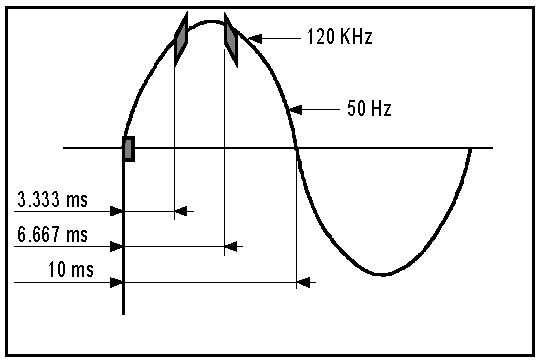
\includegraphics{imagenes/image_x10.jpg}
	\caption{Ejemplo de modulacion de onda X-10}
	\label{fig:modulacionx10}
\end{figure}


La onda modulada actúa a lo largo de los ciclos como generadora de código
digital. El protocolo X-10 se sirve de 11 ciclos de tensión alterna de 220 VAC, la
misma de red, para insertar o no en cada ciclo la señal de 120 Khz. En general,
la existencia de esta señal representa un uno y su ausencia un cero. Los
primeros cuatro bits representan el código de inicio. Casi todos los protocolos
tienen unos bits en su comienzo, que se utilizan para la sincronización y el
alineamiento del transceptor, con un número codificado en binario que define al
protocolo y lo mismo ocurre en el X-10.


La señal de 50 Hz (corriente) alimenta a los receptores y la señal de 120
Khz (de información) se filtra y es recibida por los receptores.


El protocolo X-10 usa una modulación muy sencilla comparada con las
que usan otros protocolos de control por ondas portadoras. El transceptor X-10
est\'a pendiente de los pasos por cero de la onda senoidal de 50 Hz típica de la
alimentación eléctrica (60 Hz en Estados Unidos) para insertar un instante
despuésuna r\'afaga muy corta de señal en una frecuencia fija.


Se puede insertar esta señal en los semiciclos positivos y negativos de
la onda senoidal. La codificación de un bit uno o de un bit cero, depende de
cómo seinyecte esta señal en los dos semiciclos. Un uno binario se representa
por un pulso de 120 KHz durante uno ms y el cero binario se representa por la
ausencia de ese pulso de 120 KHz. En un sistema trif\'asico el pulso de un ms
se transmite tres veces para que coincida con el paso por el cero en cada una
de las tres fases.


Por lo tanto, el Tiempo de bit coincide con los 20 ms que dura el ciclo de
la señal, de forma que la velocidad binaria de 50 bps (bit/s) viene impuesta por
la frecuencia de la red eléctrica que tenemos en Europa (50 Hz). En Estados
Unidos la velocidad binaria son 60 bps (bit/s), ya que su frecuencia de la red
eléctrica es de 60 Hz.


La transmisión completa de una orden X-10 necesita once ciclos de
corriente. Esta trama se divide en tres campos de información:
\begin{enumerate}
	\item Dos ciclos representan el código de inicio.
	\item Cuatro ciclos representan el código de casa (letras A-P).
	\item Cinco ciclos representan o bien el código numérico (1-16) o bien
el código de función (encender, apagar, aumento de intensidad,
etc.)
\end{enumerate}


En la figura \ref{fig:trama_x10} se puede observar que inmediatamente
después de los primeros dos ciclos que representan el código de inicio,
cuatro bits, se tiene dos bloques: el primero representa el llamado código
de casa y comprende otros cuatro bits y el segundo representa el
llamado código de unidad y comprende los últimos cinco bits del
protocolo.

\begin{figure}[htbp]
	\centering
		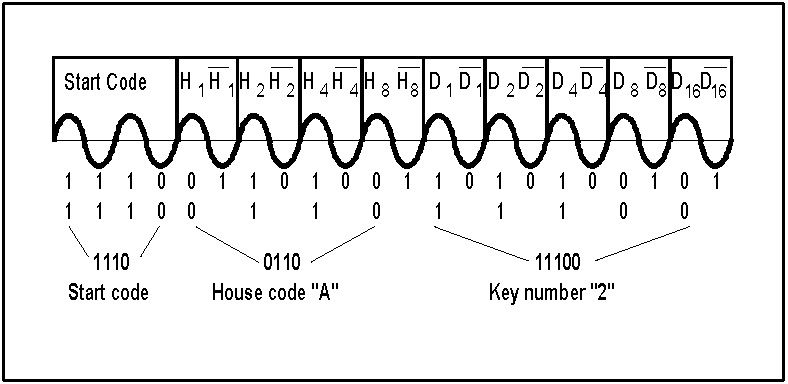
\includegraphics{imagenes/trama_x10.jpg}
	\caption{Trama de una peticion en X-10}
	\label{fig:trama_x10}
\end{figure}


La forma de extraer la codificación en estos dos últimos bloques
es ligeramente distinta a como se hace en el primero. Mientras en el
código de inicio se toman en cuenta los semiciclos, en el código de casa
y en el de unidad sólo se extrae la información del primer semiciclo de
cada ciclo, aprovechando el segundo semiciclo para transmitir la señal
del primero pero complementada. Esto se hace por seguridad. Así, en un
ciclo de cualquiera de estos dos últimos bloques no puede haber dos
ceros o dos unos seguidos, sí entre ciclos distintos.


Para aumentar la fiabilidad del sistema, esta trama (código de
inicio, código de casa y código de función o numérico) se transmite
siempre dos veces, separ\'andolas por tres ciclos completos de corriente.
Hay una excepción, en funciones de regulación de intensidad se
transmiten de forma continuada (por lo menos dos veces) sin separación
entre tramas.


La nomenclatura Hn-Dn corresponde, respectivamente, al código
de casa y al código de unidad y todas las combinaciones posibles se
indican en la tabla \ref{tab:codigosx10}.

\begin{table}[htbp]
\centering
\begin{tabular}{cccccccccccc}
\toprule
\multicolumn{5}{c}{Codigos de casa} &  &\multicolumn{6}{c}{Códigos de unidad o dispositivo}\\ \toprule
  & H1 & H2 & H4 & H8 &    &    & D1 & D2 & D4 & D8 & D16\\ \midrule
A & 0  & 1  & 1  & 0  &    & 1  & 0  & 1  & 1  & 0  & 0\\
B & 1  & 1  & 1  & 0  &    & 2  & 1  & 1  & 1  & 0  & 0\\
C & 0  & 0  & 1  & 0  &    & 3  & 0  & 1  & 1  & 0  & 0\\
D & 1  & 0  & 1  & 0  &    & 4  & 1  & 0  & 1  & 0  & 0\\
E & 0  & 0  & 0  & 1  &    & 5  & 0  & 0  & 0  & 1  & 0\\
F & 1  & 0  & 0  & 1  &    & 6  & 1  & 0  & 0  & 1  & 0\\
G & 0  & 1  & 0  & 1  &    & 7  & 0  & 1  & 0  & 1  & 0\\
H & 1  & 1  & 0  & 1  &    & 8  & 1  & 1  & 0  & 1  & 0\\
I & 0  & 1  & 1  & 1  &    & 9  & 0  & 1  & 1  & 1  & 0\\
J & 1  & 1  & 1  & 1  &    & 10 & 1  & 1  & 1  & 1  & 0\\
K & 0  & 0  & 1  & 1  &    & 11 & 0  & 0  & 1  & 1  & 0\\
L & 1  & 0  & 1  & 1  &    & 12 & 1  & 0  & 1  & 1  & 0\\
M & 0  & 0  & 0  & 0  &    & 13 & 0  & 0  & 0  & 0  & 0\\
N & 1  & 0  & 0  & 0  &    & 14 & 1  & 0  & 0  & 0  & 0\\
O & 0  & 1  & 0  & 0  &    & 15 & 0  & 1  & 0  & 0  & 0\\
P & 1  & 1  & 0  & 0  &    & 16 & 1  & 1  & 0  & 0  & 0\\ \bottomrule \addlinespace
\multicolumn{12}{c}{Funciones}\\ \midrule
\multicolumn{7}{c}{Apagar todas las unidades} & 0 & 0 & 0 & 0 & 1 \\
\multicolumn{7}{c}{Encender todas las luces}  & 0 & 0 & 0 & 1 & 1 \\
\multicolumn{7}{c}{Encender}                  & 0 & 0 & 1 & 0 & 1 \\
\multicolumn{7}{c}{Apagar}                    & 0 & 0 & 1 & 1 & 1 \\
\multicolumn{7}{c}{Atenuar intensidad}        & 0 & 1 & 0 & 0 & 1 \\
\multicolumn{7}{c}{Aumentar intensidad}       & 0 & 1 & 0 & 1 & 1 \\ \bottomrule \addlinespace
\multicolumn{12}{c}{Codigos de función para controladores OEM}\\ \midrule 
\multicolumn{7}{c}{Apagar todas las luces}    & 0 & 1 & 1 & 0 & 1 \\
\multicolumn{7}{c}{Codigo extendido}          & 0 & 1 & 1 & 1 & 1 \\
\multicolumn{7}{c}{Peticion de saludo}        & 1 & 0 & 0 & 0 & 1 \\
\multicolumn{7}{c}{Aceptacion de saludo}      & 1 & 0 & 0 & 1 & 1 \\
\multicolumn{7}{c}{Atenuacion preestablecida} & 1 & 0 & 1 & X & 1 \\
\multicolumn{7}{c}{Datos extendidos}          & 1 & 1 & 0 & 0 & 1 \\
\multicolumn{7}{c}{Estado = on}               & 1 & 1 & 0 & 1 & 1 \\
\multicolumn{7}{c}{Estado = off}              & 1 & 1 & 1 & 0 & 1 \\
\multicolumn{7}{c}{Peticion de estado}        & 1 & 1 & 1 & 1 & 1 \\ \bottomrule
\end{tabular}
\caption{Códigos X-10}
\label{tab:codigosx10}
\end{table}




El sistema X-10 es de una topología flexible, tanto, que es posible
sustituir elementos convencionales por dispositivos X-10 y un emisor puede
activar los distintos receptores. En la figura \ref{fig:estructura_x10} se muestra un ejemplo de estructura de un sistema X-10:

\begin{figure}[htb]
	\centering
		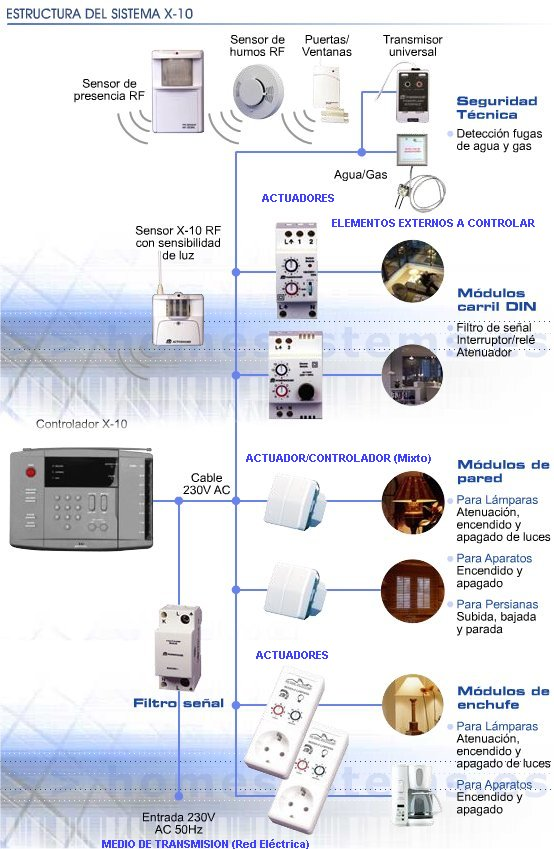
\includegraphics[width=0.8\textwidth]{imagenes/estructura_x10.jpg}
	\caption{Estructura de un sistema X-10}
	\label{fig:estructura_x10}
\end{figure}





Ademas el cambio de direccionamiento es sencillo ya que a todos los
elementos se les puede cambiar su dirección física manipulando el propio
dispositivo. Cada elemento lleva una o dos ruedas giratorias susceptibles de
ser manipuladas con un simple destornillador, con lo que se puede determinar
el código de casa y el código de unidad. Por ejemplo se podrían cofigurar dos o
mas elementos con el mismo direccionamiento y activar los a la vez, en vez de
activarlos uno a uno.


En conclusión, el protocolo X-10 es un sistema flexible, ampliable, de
f\'acil instalación y económico. En su contra tiene la poca fiabilidad de sus
comunicaciones, debido a que casi cualquier aparato eléctrico provoca
interferencias en la línea eléctrica, y la baja velocidad de transmisión datos.
\clearpage
\subsection{LonWorks}
El protocolo LONWORKS, que también es conocido como LonTalk o el
est\'andar de redes ANSI/EIA 709.1, es el corazón del sistema LONWORKS.


El protocolo provee de un conjunto de servicios de comunicación que
permite al programa de aplicación de un dispositivo enviar y recibir mensajes
de otros dispositivos sobre una red de control sin necesidad de conocer la
topología de la red ni los nombres, direcciones o funciones de otros
dispositivos. Los servicios de soporte para la gestión de la red permiten a las
herramientas de gestión remota de la red interactuar con los dispositivos de la
red, incluyendo:
\begin{itemize}
	\item Reconfiguración de las direcciones y par\'ametros.
	\item Descarga de programas de aplicación.
	\item Reporte de problemas de red.
	\item Arrancar, parar y/o resetear programas de aplicación de dispositivos
	\end{itemize}

El protocolo LONWORKS es un protocolo basado en paquetes caracterizado por la forma en la que se comunican los nodos entre si. Todo los nodos est\'an en igualdad de condiciones, de forma que no existe el concepto de cliente-servidor.



Adem\'as contempla una arquitectura de capas basada en el modelo OSI para
asegurarse que cumple con los requerimientos específicos de un sistema de
control de manera fiable y robusta.


El protocolo implementa las siete capas del modelo OSI:
\begin{figure}[htbp]
	\centering
		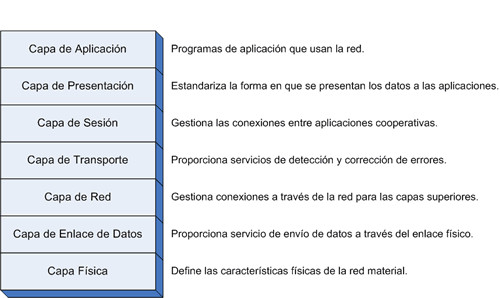
\includegraphics[width=0.80\textwidth]{imagenes/modelo_osi.jpg}
	\caption{Modelo OSI}
	\label{fig:modelo_osi}
\end{figure}



\begin{description}
	\item[Capa física] Se define el medio de transmisión. Este medio asegura que
cada bit enviado por un dispositivo fuente es recibido a todos
los dispositivos destino.
	\item[Capa de enlace]Define el método de acceso al medio y la codificación
de datos para asegurar el uso eficiente del canal de comunicaciones. La
capa de enlace define cu\'ando un dispositivo puede transmitir tramas de
datos, cómo reciben los dispositivos dichas tramas y detecta errores en
la transmisión.
	\item[Capa de red]Define cómo se mandan los paquetes de mensaje desde
un dispositivo fuente a uno o m\'as dispositivos destino. En esta capa se
define la manera de nombrar y direccionar los dispositivos de manera
que asegure la correcta entrega de paquetes, adem\'as de definir cómo
se realiza el ruteado de los mensajes en los diferentes canales de
comunicación.
	\item[Capa de transporte]Asegura una entrega fiable de paquetes. Los
mensajes pueden ser intercambiados usando un servicio de
reconocimiento, de manera que el dispositivo emisor, esperar\'a a recibir
un “reconocimiento” del receptor y reenviar el mensaje si el
reconocimiento no es recibido. En esta capa también se define cómo
detectar mensajes duplicados y cómo son rechazados si un mensaje es
reenviado por falta de reconocimiento ‘acknowledgement’.
	\item[Capa de sesión]Añade control al intercambio de datos entre las capas
inferiores. Soporta las acciones remotas para que un cliente pueda
enviar peticiones a un servidor remoto y recibir la respuesta a esta
petición.También chequea la autorización de los dispositivos emisores.
	\item[Capa de presentación]Añade una estructura a los datos intercambiados
entre las capas inferiores definiendo la codificación de los datos de
mensaje. Los mensajes pueden ser codificados como variables de
red, mensajes de aplicación, o tramas externas. La codificación
interoperable de las variables de red se consigue con el est\'andar de los
tipos devariables de red (SNVTs).
	\item[Capa de aplicación]aporta compatibilidad de aplicaciones a los datos
intercambiados por las otras capas. Esta capa también define un
protocolo de transferencia que es usado para transferir cadenas de
datos entre las distintas aplicaciones.
\end{description}

Todas las comunicaciones consisten en el intercambio de uno o m\'as paquetes entre dispositivos. Cada paquete es un número variable de bytes y contiene una representación de los datos requeridos para cada una de las siete capas. En LONWORKS, esta representación de paquetes es muy corta, minimizando el coste de la implementación de cada dispositivo.


Para poder comunicar, cada dispositivo conectado a un canal, estar\'a siempre observando los paquetes sobre el canal para ver si alguno lleva su dirección. En caso afirmativo, mirar\'a si es un paquete de datos para su aplicación o si es un paquete de gestión. En caso de que fuera un paquete de datos de aplicación, estos datos son transferidos al programa de aplicación y en caso de que sea necesario, se responder\'a al dispositivo emisor con un mensaje de autenticación o reconocimiento.


Hasta hace muy pocos años, el protocolo LONWORKS estaba solo disponible embebido en el ‘Neuron Chip’. Esto aseguraba una aplicación consistente para todos los fabricantes. Ahora que hay un gran número de dispositivos compatibles instalados, Echelon Corporation ha publicado el protocolo LONWORKS y lo ha convertido en un est\'andar abierto dentro de la ANSI/EIA709.1 Est\'andar de Redes de Control. El protocolo es, por tanto, de libre disposición para todo el mundo. Aun asi, la manera m\'as económica y efectiva de implementar este protocolo sigue siendo con la utilización del Neuron Chip.

Este Neuron Chip fue creado por Echelon, el nombre le fue puesto para hacer una similitud con el cerebro humano, ya que esta formado por neuronas que, a diferencia de un control 
centralizado, reparten el control en millones de ellas,estando interconectadas y cada una proveyendo información por múltiples rutas. Cada una de ellas suele estar dedicada a una función específica, pero la pérdida de una de ellas no implica la pérdida de funcionalidad del sistema. El ‘Neuron Chip’ incluye las primeras 6 capas del modelo OSI/ISO, por lo que el desarrollador sólo tiene que preocuparse del programa de aplicación. Es un dispositivo semiconductor especialmente diseñado para proveer inteligencia y capacidades de comunicación a dispositivos de control de bajo coste. Incluye 3 procesadores, 2 para comunicación y 1 para el procesamiento de la aplicación. Los fabricantes de dispositivos proveen el código de aplicación que corre en el‘Neuron Chip’ y los dispositivos de E/S para ser conectados al el.


El Neuron Chip tiene en su interior una memoria ROM que contiene un sistema operativo completo, llamado ‘Neuron Chip Firmware’, incluyendo el protocolo LONWORKS y una librería de funciones de E/S (Entrada/Salida). El chip tiene una memoria no vol\'atil para los datos de configuración y para el programa de aplicación.


Cada dispositivo LONWORKS unido a la red, normalmente contiene un ‘Neuron Chip’ y un transceptor. Dependiendo de la función del dispositivo, puede haber también sensores y actuadores embebidos e interfaces de entrada y salida a sensores y actuadores. El programa de aplicación que es ejecutado por el ‘Neuron Chip’ puede residir permanentemente en una ROM o puede ser descargado sobre la red en una memoria no vol\'atil de lectura/escritura (NVRAM, flash PROM, o EEPROM).


El trabajo de la mayor parte de los dispositivos en una red LONWORKS es sensorizar y controlar el estado de los componentes que forman el sistema físico. Estos son llamados dispositivos de control LONWORKS.


El programa de aplicación de un dispositivo, puede enviar y recibir valores dela red, realizar procesamiento de los datos (linearización, escalado,…) de lasvariables sensorizadas y procesar datos de lógicas de control como lazos de control PIDs.

\subsection{KNX}
La asociación KNX o Konnex nace en 1999 como la iniciativa de tres organizaciones, que ya llevaban años en el mercado europeo, aunque con tecnologías bien diferentes, así como objetivos y \'ambitos de actuación complementarios. Estas organizaciones son: EIBA, BatiBUS y EHS.


En la actualidad, la organización que m\'as ha realizado para conseguir un protocolo común ha sido EIB, por lo que el protocolo es también conocido como KNX-EIB. A día de hoy, KNX es el único protocolo certificado libre que existe especializado en la domótica.


Los medios de comunicación que usa el protocolo KNX son los siguientes: 
\begin{itemize}
	\item Par trenzado (TP1): aprovechando la norma EIB equivalente.
	\item Par trenzado (TP0): aprovechando la norma Batibus equivalente. 
	\item Ondas Portadoras (PL100): aprovechando la norma EIB equivalente.
	\item Ondas Portadoras (PL132): aprovechando la norma EHS equivalente. 
	\item Ethernet: aprovechando la norma EIB.net. 
	\item Radiofrecuencia: aprovechando la norma EIB.RF
\end{itemize}
La elección de un medio de transmisión u otro depender\'a del tipo de edificio y de las instalaciones con las que éste cuente. Así, si el edificio es de nueva construcción el par trenzado es quiz\'as el medio m\'as óptimo, mientras que si el edificio est\'a ya construido es posible que interese m\'as el uso de la línea de potencia o radiofrecuencias.


En el sistema KNX la transmisión de las señales se hace a través de un cable o bus al que est\'an conectados todos los dispositivos. El bus permite que todos los componentes de las instalaciones domóticas estén intercomunicados entre sí, de esta forma, es posible que cualquier componente de órdenes a cualquier otro, independientemente de la distancia entre ellos y su ubicación. 


La unidad de instalación mas pequeña la forma la línea. Una línea consta de un m\'aximo de cuatro segmentos de línea, cada uno de los cuales puede disponer de 64 componentes del bus (256 elementos por linea). Mediante el uso de acopladores de línea es posible unir hasta 15 lineas en una zona (3840 elementos por zona). Cada línea dispondr\'a de su fuente de alimentación EIB, y estar\'a separada galv\'anicamente del resto de líneas. Esto es importante, porque supone que si se produce un fallo en alguna línea, el resto seguir\'a funcionando normalmente. Tambien se pueden usar acopladores de zona, para unir distintas zonas a través de una línea principal, hasta un m\'aximo de 15. Con lo cual, podemos tener hasta 57600 elementos en total.

La división en zonas y líneas es muy ventajosa, ya que significa que el trafico de información local , no afecta a los datos del resto de líneas o zonas. El acoplador de línea impedir\'a el paso hacia otras líneas de datagramas cuyos destinos sena elementos de su línea. Y, al mismo tiempo ignorara aquellos datagramas provenientes de otras líneas o zonas que no conciernan a elementos de su línea. Esto posibilitara la comunicación simultanea en multiples líneas independientes unas de otras y sin congestionar la red.


Gracias a la división jerarquica en zonas y líneas, la instalación de un sistema EIB resulta f\'acilmente comprensible a la hora de la puesta en marcha, el diagnostico y las tareas de mantenimiento. Comenzando por unas pocas líneas al principio de la instalación, es posible ampliar paso a paso el sistema cuando y como las nuevas necesidades o usos de las instalaciones asi lo requieran.


En la figura \ref{fig:estructuraknx} podemos ver un ejemplo de conexión de líneas y \'areas:

\begin{figure}[ht]
	\centering
		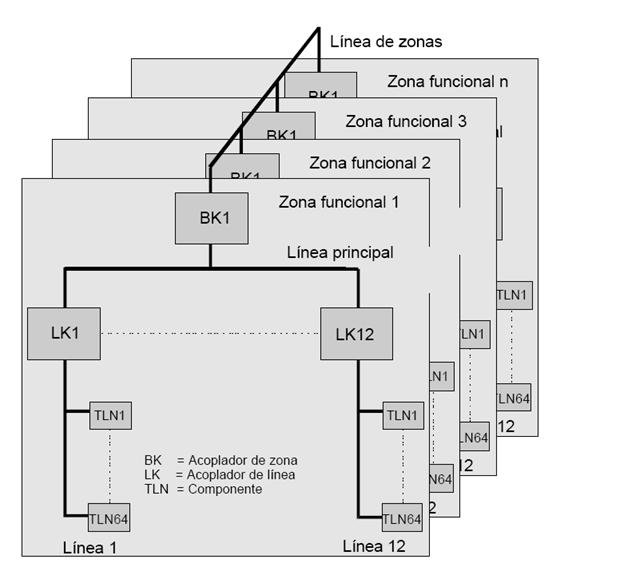
\includegraphics[width=0.8\textwidth]{imagenes/Acopladores-Knx.jpg}
	\caption{Estructura KNX}
	\label{fig:estructuraknx}
\end{figure}


Una vez visto cómo se estructura, vamos a ver cómo se envían los datos el protocolo KNX. La información que circula por el bus, como por ejemplo las ordenes de conmutación, es intercambiada entre los componentes conectados al bus en forma de datagramas o telegramas. La información se transmite de forma simétrica en el bus, es decir, como una diferencia de potencial entre los dos hilos y no referida a tierra, como muestra la figura \ref{fig:transmisionknx}. De esta forma, las interferencias o ruido, al afectar a ambos hilos de forma similar, influyen en menor grado en la transmisión de la información. 


\begin{figure}[ht]
	\centering
		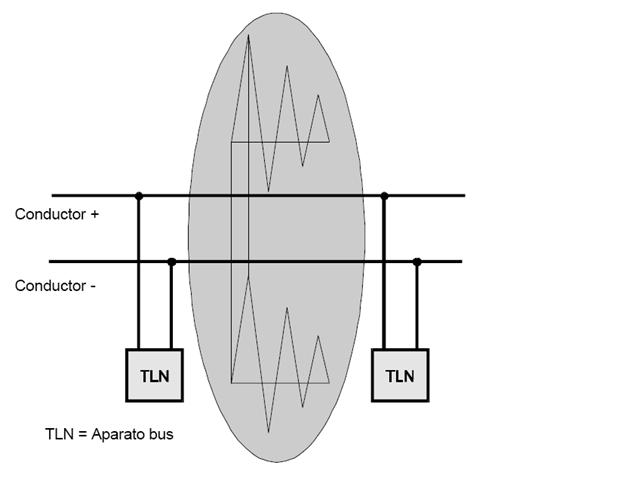
\includegraphics[width=0.8\textwidth]{imagenes/topologia-knx.jpg}
	\caption{Transmision de la señal KNX}
	\label{fig:transmisionknx}
\end{figure}



La tasa de transmisión es de 9600 bit/s, siendo el tiempo medio de transmisión de un datagrama de unos 25 ms.


Para enviar un telegrama, lo primero que hace un dispositivo es esperar un tiempo hasta que el medio por el que va a transmitir esté libre, y una vez que esté libre espera un tiempo también para comprobar que nadie ha empezado a enviar datos. Si esto se cumple, empezaría con la transmisión y una vez terminado este envío, se espera un tiempo hasta que los dispositivos a los que se les ha enviado la información confirmen que han recibido bien el paquete. 



Aparte, cada byte de datos se agrupan formando caracteres o palabras, que adem\'as de estos datos se componen de otros bits como se puede observar en la figura \ref{fig:palabra_knx}.
\begin{figure}[htbp]
	\centering
		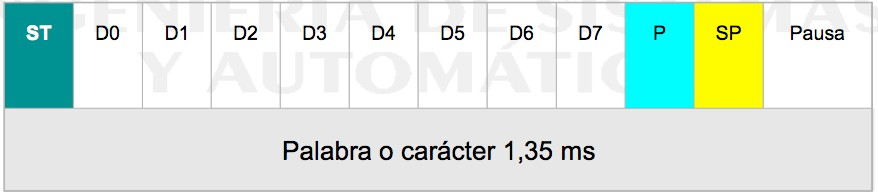
\includegraphics[width=0.80\textwidth]{imagenes/palabra_knx.jpg}
	\caption{Bits de una palabra en KNX}
	\label{fig:palabra_knx}
\end{figure}


\begin{description}
	\item[ST]Es un bit de inicio, que indica el comienzo de una nueva palabra.
	\item[P]Es el llamado bit de paridad, trabaja con paridad par y completa la suma de los bits de datos, para trabajar con dicha paridad.
	\item[SP]Es un bit de parada, e indica que la palabra o carácter ha terminado.
	\item[Pausa]Después del bit de parada se espera un tiempo de pausa equivalente a dos bits para continuar con la próxima palabra.
\end{description}

Estos caracteres van dentro de un paquete de datos, que está formado por los campos mostrados en la figura\ref{fig:campos_paq_knx}.
\begin{figure}
	\centering
		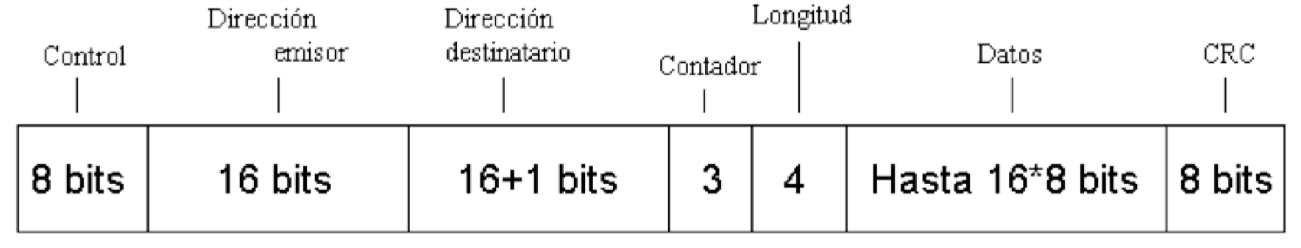
\includegraphics[width=0.80\textwidth]{imagenes/campos_paq_knx.jpg}
	\caption{Campos de un paquete KNX}
	\label{fig:campos_paq_knx}
\end{figure}


El byte de control indica la prioridad del mensaje y el inicio del mismo. Tanto la dirección del emisor como la del destinatario siguen un formato determinado, añadiendo un bit más en la dirección del destinatario que indica si se trata de una dirección física o de una dirección de grupo. El contador se utiliza para funciones de enrutamiento, contando el número de saltos que ha dado el paquete. El último byte, CRC, se utiliza para comprobar que los anteriores han sido transmitidos correctamente.


La dirección física se utiliza para identificar de manera unívoca el componente de bus, describiendo su localización dentro de la topología (zona, línea y componente) dedicando los cuatro primeros bits a la zona (15 zonas), los cuatro siguientes a la línea (15 líneas) y los ocho últimos a los componentes (256 componentes).


En caso de que esta dirección sea de grupo, la forma de crearla es diferente, y se puede hacer con dos o tres subgrupos. Los subgrupos pueden ser, por ejemplo, los siguientes:
\begin{description}
	\item[Grupos principales] bombillas, persianas, aire acondicionado…
	\item[Grupo intermedio] primera planta, segunda planta…
	\item[Grupo secundario] oficinas, dormitorio…
\end{description}


Para ello destinamos 4 bits al grupo principal y dependiendo de si tenemos grupo intermedio o no, 3 bits para el intermedio y 8 para el secundario o directamente 11 para el secundario. El último bit es para indicar si la dirección era de grupo o dirección física. Esto se ve mejor en la figura \ref{fig:Niveles-direccionamiento-grupo-knx}.
\begin{figure}[htbp]
	\centering
		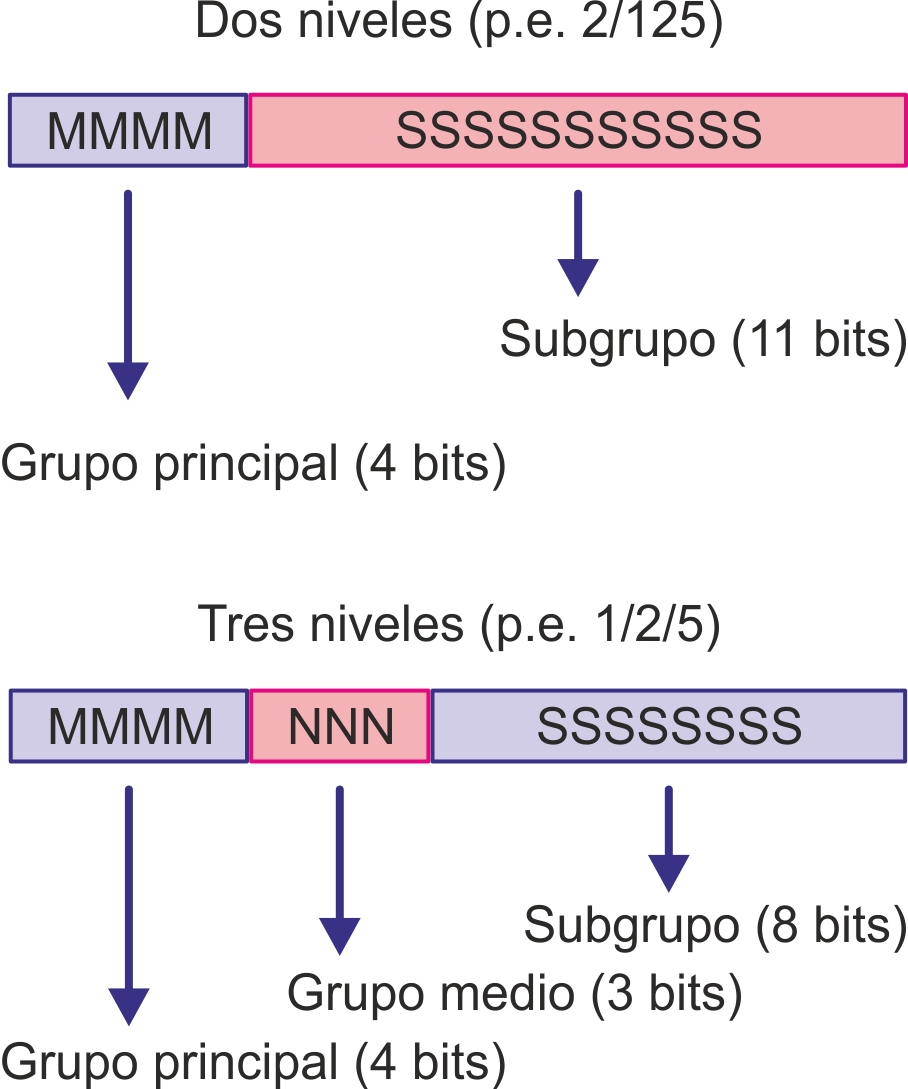
\includegraphics[width=0.80\textwidth]{imagenes/Niveles-direccionamiento-grupo-knx.png}
	\caption{Direccionamiento en KNX}
	\label{fig:Niveles-direccionamiento-grupo-knx}
\end{figure}



Las direcciones de grupo son básicas para el funcionamiento del sistema ya que permiten relacionar sensores con actuadores. Además, estará permitido relacionar elementos de distintas áreas y distintas líneas, siempre y cuando se cumplan ciertas restricciones:
\begin{itemize}
	\item Los sensores sólo pueden tener asociada una dirección de grupo.
	\item Varios actuadores pueden tener asociada una misma dirección de grupo. Cada vez que dicha dirección sea direccionada, se activarán todos los actuadores asociados a ella, respondiendo todos ellos al mismo telegrama.
	\item Los actuadores pueden estar asociados a varias direcciones de grupos, es decir, un actuador puede estar asociado a uno o más de un sensor.
\end{itemize}


El funcionamiento será el siguiente: el emisor envía un telegrama al bus. Este telegrama llega a todos los dispositivos, lo cuales leen el campo dirección de grupo y sólo los que posean dicha dirección responden de la forma oportuna.


Una vez los dispositivos se pueden interconectar, sólo hace falta que se entiendan entre ellos. Para ello, es preciso que se comuniquen en el mismo “lenguaje”. Existen diferentes tipos de variables para transmitir los datos y están todas definidas dentro del EIS (EIB Interworking Standard). En la tabla \ref{tab:variables_eib} podemos ver un fragmento del mismo con las variables más usadas.

\begin{table}[htbp]
\centering \scriptsize
%\resizebox{\textwidth}{!} {
\begin{tabular}{cp{4cm}cp{5.5cm}}
\multicolumn{4}{c}{EIS (EIB Interworking Standard)} \\ \toprule
Nº EIS& Función EIB              & Nº de Bytes &  Descripción \\ \midrule
EIS 1 & interruptor (switching)  & 1 bit & encendido/apagado, verdadero\/falso \\ \midrule
EIS 2 & regulación (dimming)     & 4 bit & Se puede utilizar de 3 formas distintas:  como interruptor, como valor relativo  y como valor absoluto. \\ \midrule
EIS 3 & hora (time)              & 3 bytes    & día de la semana, hora, minutos y segundos. \\ \midrule
EIS 4 & fecha (date)             & 3 bytes   & Día\/mes\/año (el margen es de 1990 a 2089). \\ \midrule
EIS 5 & valor (value)            & 2 bytes  & Para enviar valores físicos con representación  S,EEEE,MMMMMMMMMMM \\ \midrule
EIS 6 & escala (scaling) & 8 bit & Se utiliza para transmitir valores relativos  con una resolución de 8 bit. Ej. FF = 100\% \\ \midrule
EIS 7 & control motores (control drive) & 1 bit & Tiene dos usos: \ Mover, arriba\/abajo o extender\/retraer y Paso a Paso. \\ \midrule
EIS 8 & prioridad (priority) & 1 bit & Se utiliza en conjunción con EIS 1 ó EIS 7. \\ \midrule
EIS 9 & coma flotante (float value) & 4 bytes & Codifica un número en coma flotante  según el formato definido por el IEEE 754. \\ \midrule
EIS 10 & contador 16 bit (16b-counter) & 2 bytes & Representa los valores de un contador de 16 bit  (tanto con signo como sin signo). \\ \midrule
EIS 11 & contador 32 bit (32b-counter) & 4 bytes & Representa los valores de un contador de 32 bit  (tanto con signo como sin signo). \\ \midrule
EIS 12 & acceso (access) & 4 bytes & Se usa para conceder accesos a distintas funciones. \\ \midrule
EIS 13 & Carácter ASCII (Character) & 8 bit & Codifica según el formato ASCII \\ \midrule
EIS 14 & contador 8 bit (8b-counter) & 8 bit & Representa los valores de un contador de 8 bit  (tanto con signo como sin signo). \\ \midrule
EIS 15 & Cadena (Character String) & 14 bytes & Transmite una cadena de caracteres ASCII  de hasta 14 bytes. \\ \bottomrule
\end{tabular}
%}
\caption{Variables mas usadas en EIB}
\label{tab:variables_eib}
\end{table}



